% Bloque desactivado: esta figura correspondía a la agregación anterior de tres logros educativos.
\iffalse
\begin{figure}[H]
  \centering
  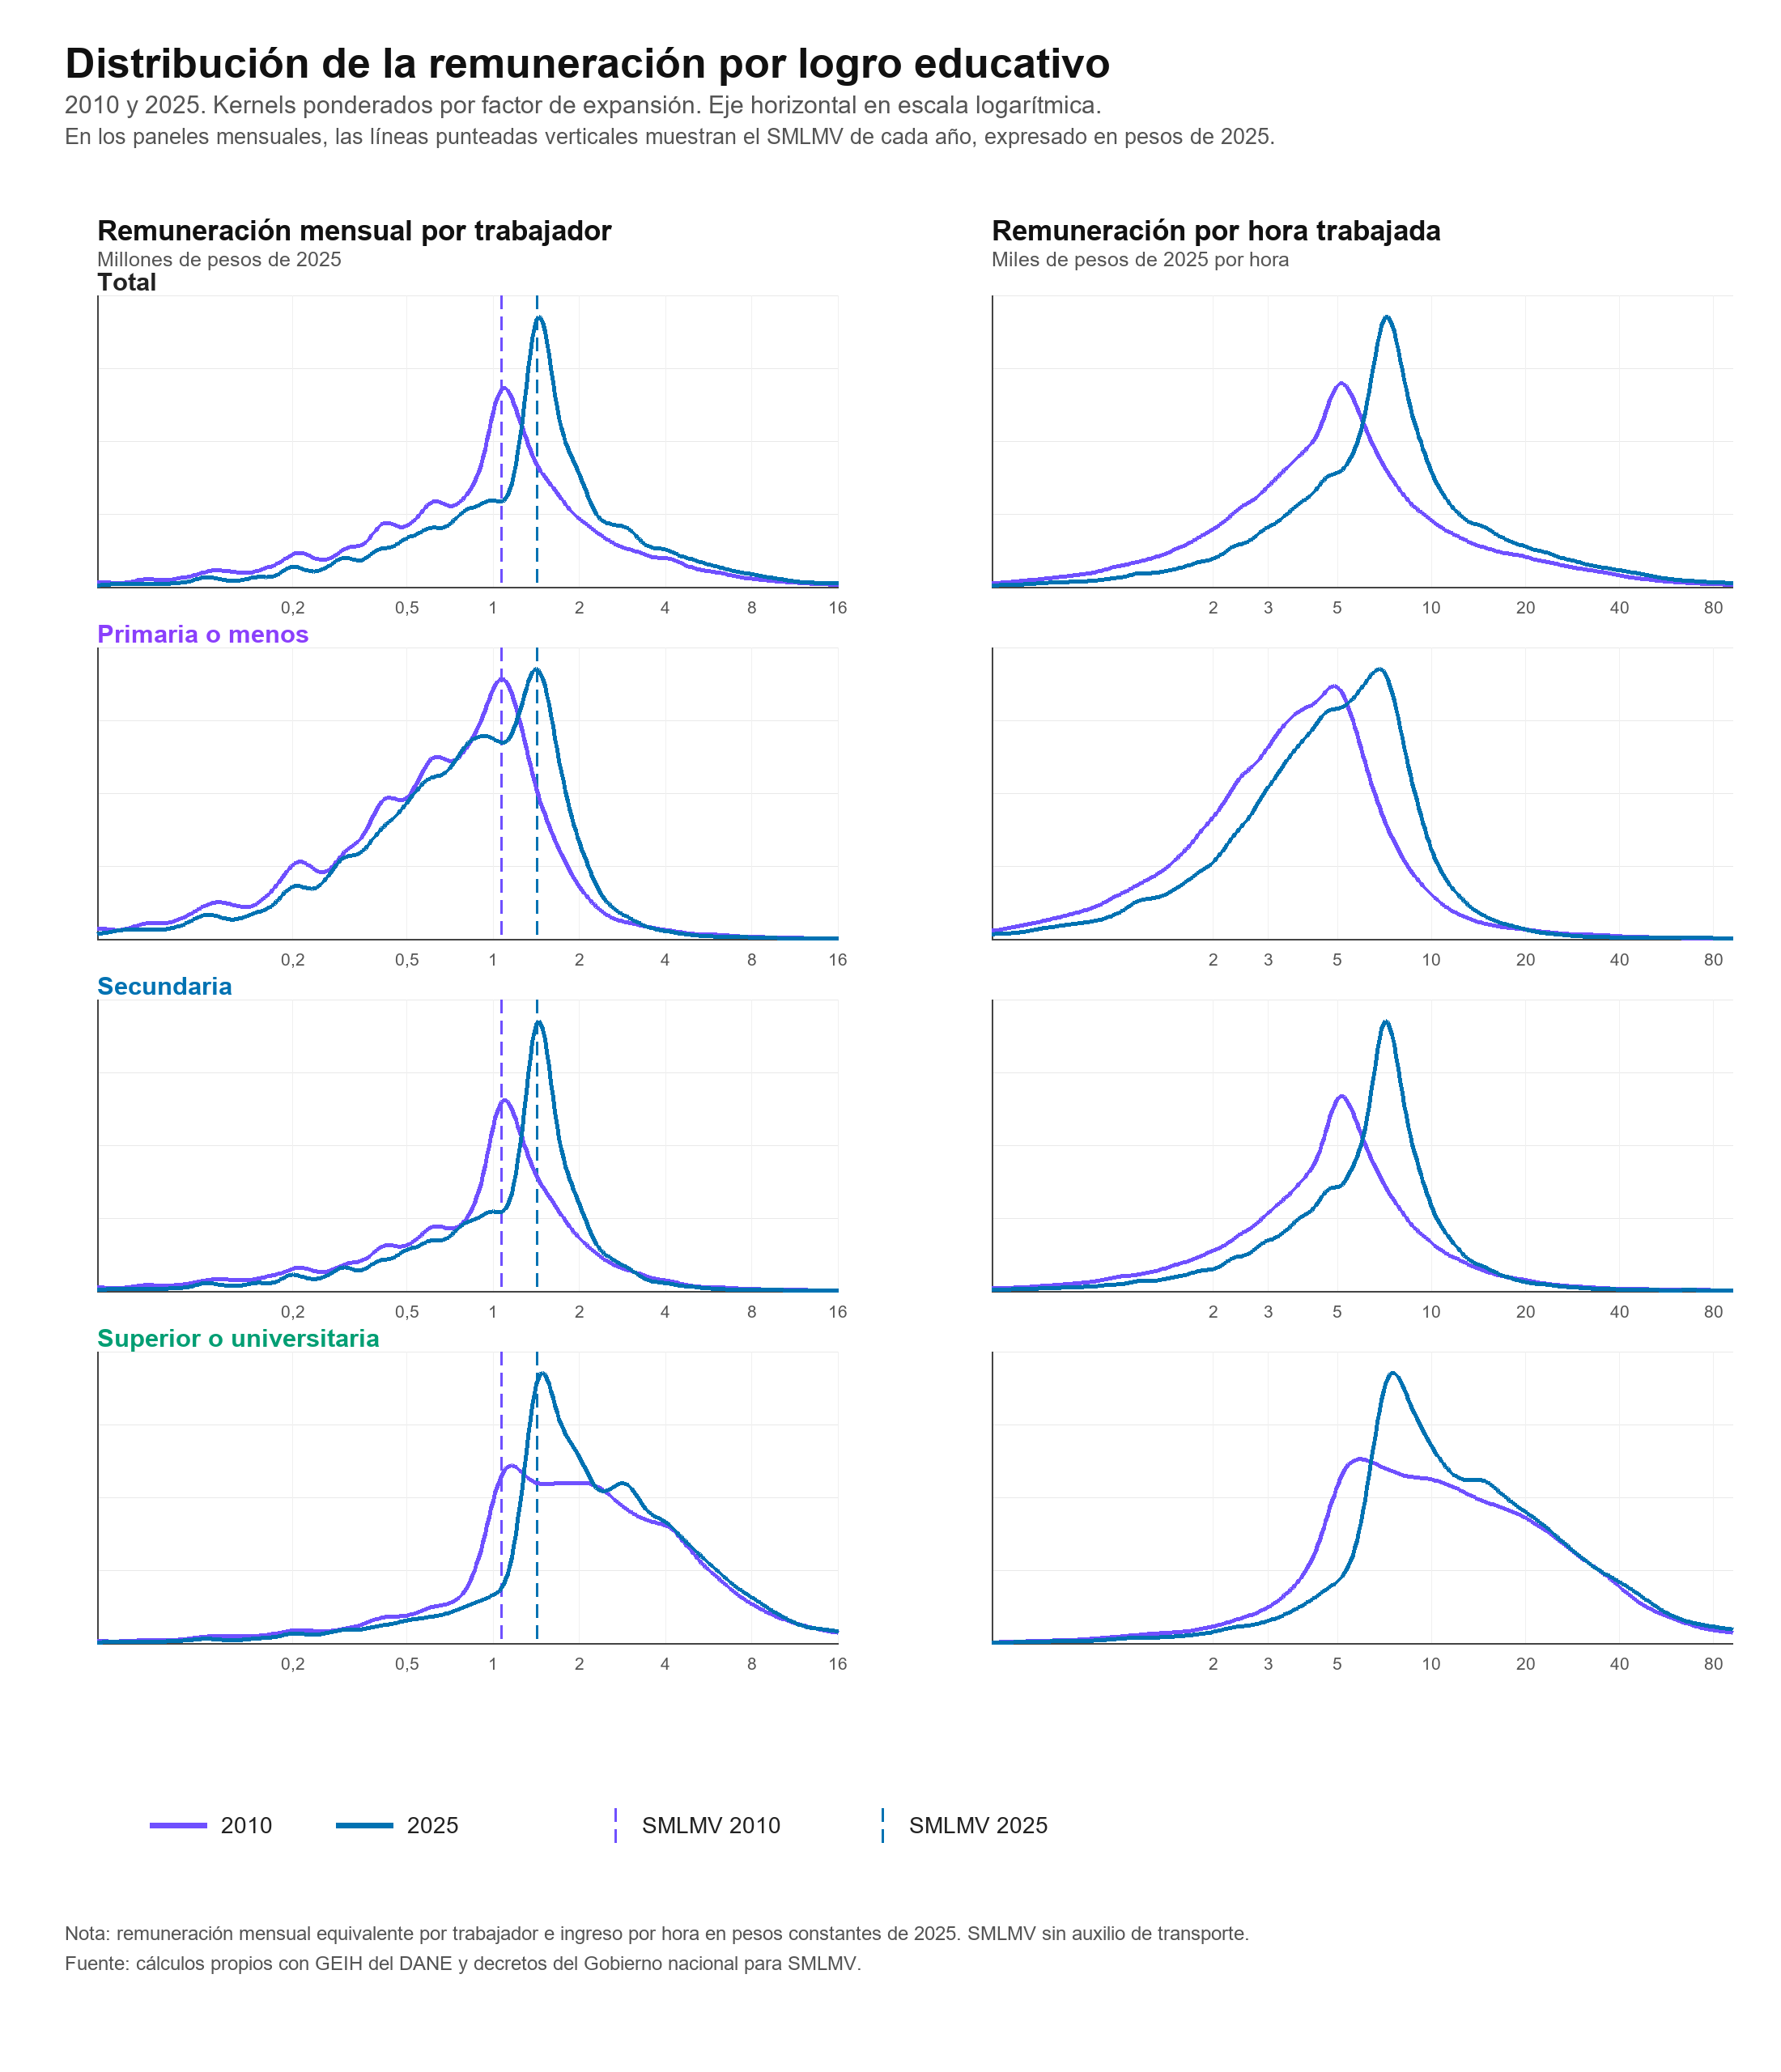
\includegraphics[width=0.98\textwidth]{Paper/figures/fig_kernel_remuneracion_educacion_comparable_2010_2025.png}
  \caption{Distribución de la remuneración laboral total y por logro educativo, 2010 y 2025}
  \label{fig:remuneracion_educacion_kernels}
  \caption*{\footnotesize Nota: distribuciones estimadas con factores de expansión. Los paneles mensuales muestran remuneración mensual equivalente por trabajador. Los paneles por hora muestran ingreso laboral por hora. El eje horizontal está en escala logarítmica. El SMLMV no incluye auxilio de transporte. Fuente: cálculos propios con GEIH del DANE y decretos del Gobierno nacional para SMLMV.}
\end{figure}
\fi

\begin{figure}[H]
  \centering
  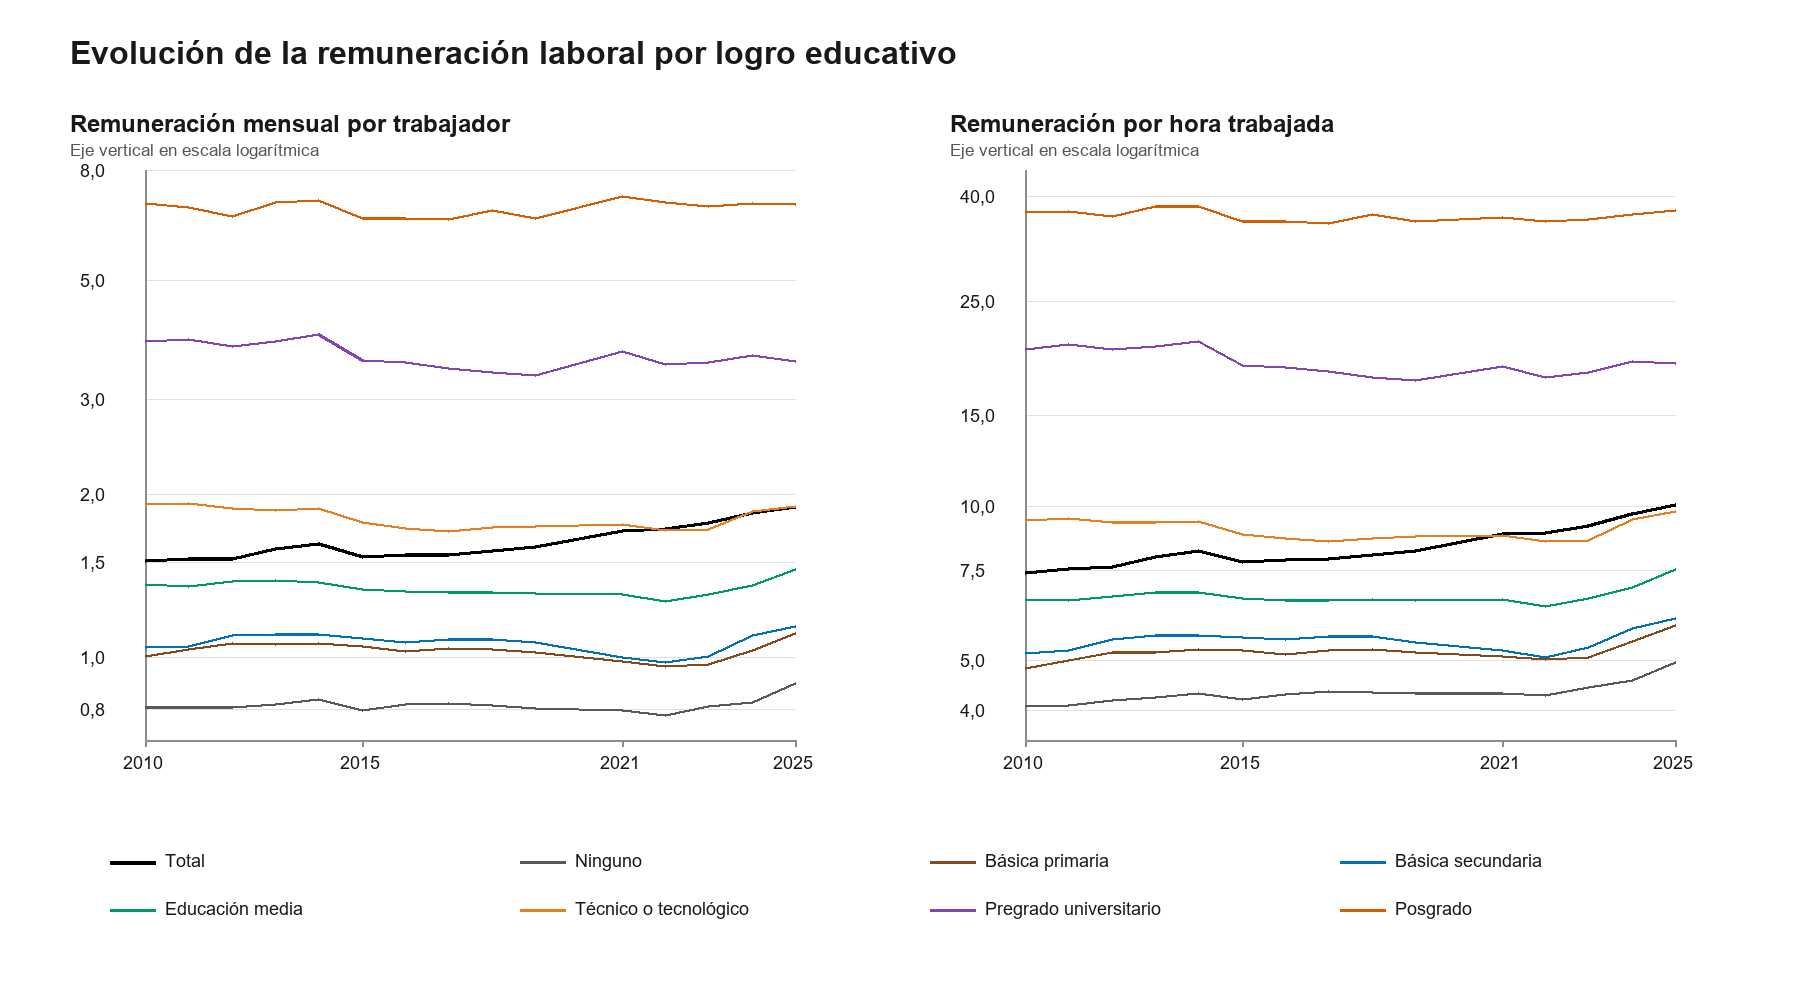
\includegraphics[width=0.98\textwidth]{Paper/figures/fig_remuneracion_educacion_series_comparables.png}
  \caption{Evolución de la remuneración laboral total y por logro educativo, 2010--2025}
  \label{fig:remuneracion_educacion_series_comparables}
  \caption*{\footnotesize Nota: el panel izquierdo muestra la remuneración mensual por trabajador en millones de pesos mensuales de 2025. El panel derecho muestra la remuneración por hora trabajada en miles de pesos de 2025. El eje vertical de ambos paneles está en escala logarítmica. La serie excluye 2020. Fuente: cálculos propios con GEIH del DANE.}
\end{figure}

% Bloque desactivado: este cuadro correspondía a la agregación anterior de tres logros educativos.
\iffalse
\begin{table}[H]
\centering
\caption{Tasas laborales por logro educativo comparable, 2010 y 2025}
\label{tab:tasas-laborales-educacion}
\begin{threeparttable}
\scriptsize
\setlength{\tabcolsep}{3.5pt}
\resizebox{\textwidth}{!}{%
\begin{tabular}{lcccccccc}
\toprule
& \multicolumn{2}{c}{Tasa de participación}
& \multicolumn{2}{c}{Tasa de ocupación}
& \multicolumn{2}{c}{Tasa de desempleo}
& \multicolumn{2}{c}{Tasa de formalidad} \\
\cmidrule(lr){2-3} \cmidrule(lr){4-5} \cmidrule(lr){6-7} \cmidrule(l){8-9}
Logro educativo
& 2010 & 2025
& 2010 & 2025
& 2010 & 2025
& 2010 & 2025 \\
\midrule
Primaria o menos
& 62,9 & 52,8
& 57,8 & 50,0
& 8,2 & 5,4
& 11,5 & 13,0 \\

Secundaria o media
& 67,1 & 64,1
& 57,4 & 57,8
& 14,4 & 9,6
& 31,3 & 36,7 \\

Superior o universitaria
& 78,3 & 74,3
& 67,9 & 67,0
& 13,3 & 10,0
& 67,5 & 76,0 \\
\bottomrule
\end{tabular}
}
\begin{tablenotes}
\scriptsize
\item \textit{Nota:} La tasa de participación se calcula como PEA/PET, la tasa de ocupación como ocupados/PET, la tasa de desempleo como desocupados/PEA y la tasa de formalidad como ocupados que cotizan a pensión sobre ocupados con clasificación válida de cotización. Las tasas se reportan en porcentaje. Los cálculos usan factores de expansión anualizados.
\end{tablenotes}
\end{threeparttable}
\end{table}
\fi

\begin{table}[H]
\centering
\caption{Tasas laborales por logro educativo detallado, 2021 y 2025}
\label{tab:tasas-laborales-educacion-detallada-2021-2025}
\begin{threeparttable}
\scriptsize
\setlength{\tabcolsep}{3.5pt}
\resizebox{\textwidth}{!}{%
\begin{tabular}{lccccccccc}
\toprule
& \multicolumn{3}{c}{Tasa de participación}
& \multicolumn{3}{c}{Tasa de ocupación}
& \multicolumn{3}{c}{Tasa de desempleo} \\
\cmidrule(lr){2-4} \cmidrule(lr){5-7} \cmidrule(lr){8-10}
Logro educativo
& 2021 & 2025 & Dif.
& 2021 & 2025 & Dif.
& 2021 & 2025 & Dif. \\
\midrule
Preescolar o ninguno
& 40,6 & 40,8 & 0,2
& 38,1 & 39,0 & 1,0
& 6,2 & 4,3 & -1,9 \\

Básica primaria
& 42,9 & 45,2 & 2,3
& 38,7 & 43,0 & 4,3
& 9,8 & 4,9 & -4,9 \\

Básica secundaria
& 53,4 & 55,4 & 2,0
& 48,7 & 52,4 & 3,7
& 9,0 & 5,5 & -3,4 \\

Media académica
& 51,3 & 55,1 & 3,8
& 43,9 & 50,3 & 6,4
& 14,5 & 8,7 & -5,8 \\

Media técnica
& 65,0 & 67,5 & 2,5
& 54,2 & 60,9 & 6,7
& 16,6 & 9,9 & -6,8 \\

Normalista
& 66,0 & 67,9 & 1,9
& 54,1 & 60,1 & 5,9
& 18,0 & 11,5 & -6,4 \\

Técnica profesional
& 51,5 & 50,7 & -0,8
& 42,9 & 42,5 & -0,4
& 16,7 & 16,1 & -0,6 \\

Tecnológica
& 74,1 & 74,0 & -0,1
& 60,6 & 65,3 & 4,6
& 18,2 & 11,8 & -6,4 \\

Universitaria
& 76,8 & 76,0 & -0,8
& 63,6 & 68,0 & 4,4
& 17,2 & 10,5 & -6,7 \\

Especialización
& 69,2 & 70,6 & 1,5
& 59,7 & 63,2 & 3,5
& 13,8 & 10,6 & -3,2 \\

Maestría
& 84,6 & 85,3 & 0,7
& 79,8 & 80,6 & 0,8
& 5,6 & 5,4 & -0,2 \\

Doctorado
& 89,4 & 90,1 & 0,7
& 85,8 & 86,4 & 0,5
& 4,0 & 4,2 & 0,2 \\
\bottomrule
\end{tabular}
}
\begin{tablenotes}
\scriptsize
\item \textit{Nota:} La tasa de participación se calcula como PEA/PET, la tasa de ocupación como ocupados/PET y la tasa de desempleo como desocupados/PEA. Las diferencias están expresadas en puntos porcentuales. Los cálculos usan factores de expansión anualizados.
\end{tablenotes}
\end{threeparttable}
\end{table}


% Bloque desactivado: no se referencia en el cuerpo del documento.
\iffalse
\begin{table}[H]
\centering
\caption{Estadísticos descriptivos de la remuneración laboral por logro educativo, 2010 y 2025}
\label{tab:estadisticos_remuneracion_educacion}
\begingroup
\setlength{\tabcolsep}{3.5pt}
\scriptsize
\begin{tabular}{@{}p{3.1cm}rrrrrr@{}}
\toprule
\multicolumn{7}{@{}l}{\textbf{Panel A. Remuneración mensual por trabajador (miles de pesos mensuales de 2025)}} \\
Logro educativo & Año & Media & Mediana & Desv. est. & Mín. & Máx. \\
\midrule
Primaria o menos & 2010 & 878 & 726 & 4.450 & $<1$ & 2.073.526 \\
Primaria o menos & 2025 & 997 & 850 & 989 & $<1$ & 80.000 \\
\addlinespace[0.25em]
Secundaria & 2010 & 1.195 & 1.068 & 1.491 & $<1$ & 207.311 \\
Secundaria & 2025 & 1.342 & 1.400 & 1.406 & $<1$ & 100.000 \\
\addlinespace[0.25em]
Superior o normalista & 2010 & 3.082 & 1.990 & 4.940 & $<1$ & 207.311 \\
Superior o normalista & 2025 & 3.228 & 2.000 & 3.921 & $<1$ & 103.000 \\
\addlinespace[0.8em]
\multicolumn{7}{@{}l}{\textbf{Panel B. Remuneración por hora trabajada (pesos de 2025 por hora)}} \\
Logro educativo & Año & Media & Mediana & Desv. est. & Mín. & Máx. \\
\midrule
Primaria o menos & 2010 & 4.561 & 3.615 & 17.679 & $<1$ & 7.975.098 \\
Primaria o menos & 2025 & 5.520 & 4.720 & 6.124 & $<1$ & 415.385 \\
\addlinespace[0.25em]
Secundaria & 2010 & 6.105 & 4.983 & 8.934 & $<1$ & 1.063.134 \\
Secundaria & 2025 & 7.106 & 6.827 & 8.151 & $<1$ & 1.153.846 \\
\addlinespace[0.25em]
Superior o normalista & 2010 & 17.042 & 10.229 & 28.960 & $<1$ & 1.794.038 \\
Superior o normalista & 2025 & 18.015 & 11.454 & 23.364 & $<1$ & 2.307.692 \\
\bottomrule
\end{tabular}
\endgroup
\caption*{\footnotesize Nota: media, mediana y desviación estándar se calculan con factores de expansión. Los mínimos y máximos son valores observados en la muestra y pueden estar afectados por valores extremos. Valores positivos menores a una unidad del panel se reportan como \(<1\). La media del Panel B describe el ingreso por hora promedio entre trabajadores. Por construcción, puede diferir de la remuneración por hora agregada del Cuadro \ref{tab:remuneracion_educacion_remuneracion}, que pondera por horas trabajadas. Fuente: cálculos propios con GEIH del DANE.}
\end{table}


\begin{table}[H]
\centering
\caption{Dispersión y masa alrededor del salario mínimo por logro educativo, 2010 y 2025}
\label{tab:masa_smlmv_educacion}
\begingroup
\setlength{\tabcolsep}{3.5pt}
\scriptsize
\begin{tabular}{@{}p{3.5cm}rrrrrr@{}}
\toprule
& \multicolumn{2}{c}{P90/P10 mensual} & \multicolumn{2}{c}{P90/P10 por hora} & \multicolumn{2}{c}{Cerca del SMLMV} \\
\cmidrule(lr){2-3} \cmidrule(lr){4-5} \cmidrule(l){6-7}
Logro educativo & 2010 & 2025 & 2010 & 2025 & 2010 & 2025 \\
\midrule
Primaria o menos & 9,2 & 7,2 & 6,3 & 5,2 & 14,2\% & 16,2\% \\
Secundaria o media & 8,3 & 5,0 & 5,4 & 4,0 & 21,0\% & 29,1\% \\
Superior o universitaria & 10,0 & 6,8 & 8,3 & 6,6 & 11,7\% & 18,4\% \\
\midrule
\textbf{Total} & 12,2 & 8,8 & 9,0 & 7,3 & 16,4\% & 22,8\% \\
\bottomrule
\end{tabular}
\endgroup
\caption*{\footnotesize Nota: cerca del SMLMV corresponde a la proporción de ocupados cuya remuneración mensual equivalente está entre 0,9 y 1,1 veces el salario mínimo legal mensual vigente del año, ambos expresados en pesos de 2025. Cálculos ponderados con factores de expansión. Fuente: cálculos propios con GEIH del DANE y decretos del Gobierno nacional para SMLMV.}
\end{table}

\fi

% Bloque desactivado: no se referencia en el cuerpo del documento.
\iffalse
\begin{figure}[H]
  \centering
  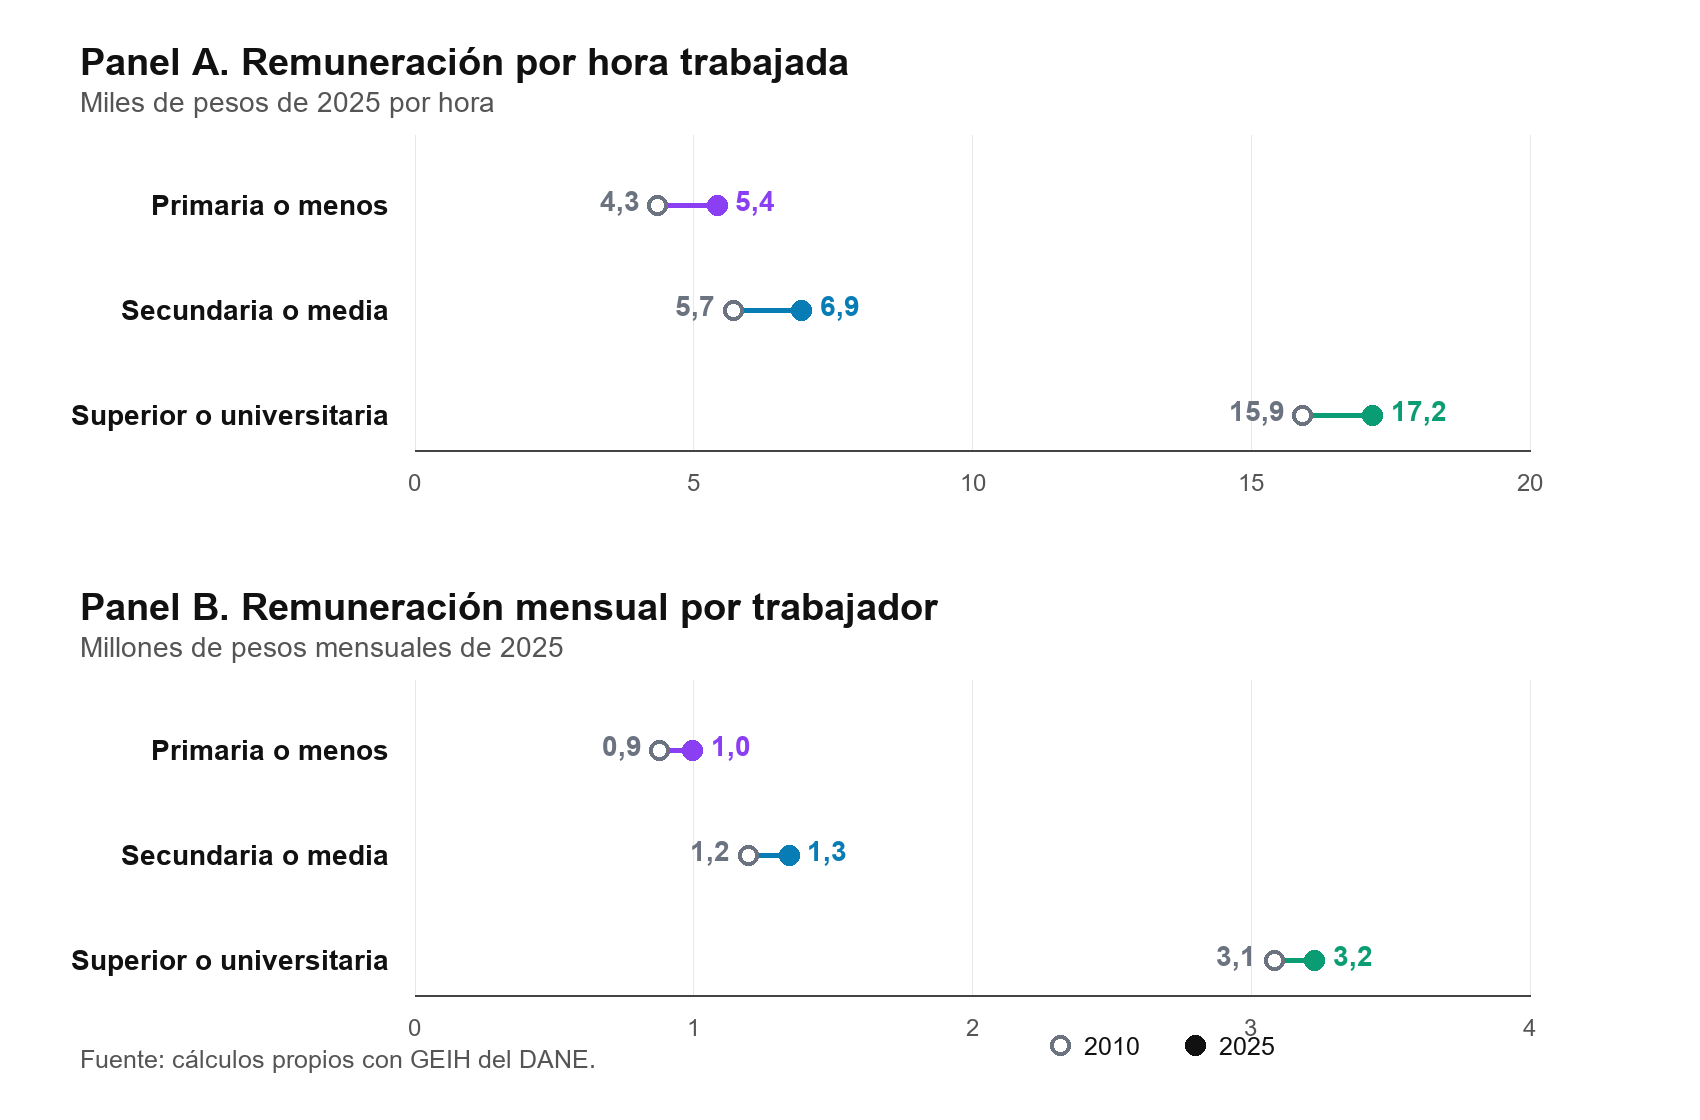
\includegraphics[width=0.98\textwidth]{Paper/figures/fig_remuneracion_educacion_niveles_2025.png}
  \caption{Remuneración laboral por logro educativo, 2010 y 2025}
  \label{fig:remuneracion_educacion_niveles_2025}
  \caption*{\footnotesize Nota: los círculos abiertos corresponden a 2010 y los círculos llenos a 2025. Pesos constantes de 2025. Fuente: cálculos propios con GEIH del DANE.}
\end{figure}
\fi

\begin{figure}[H]
  \centering
  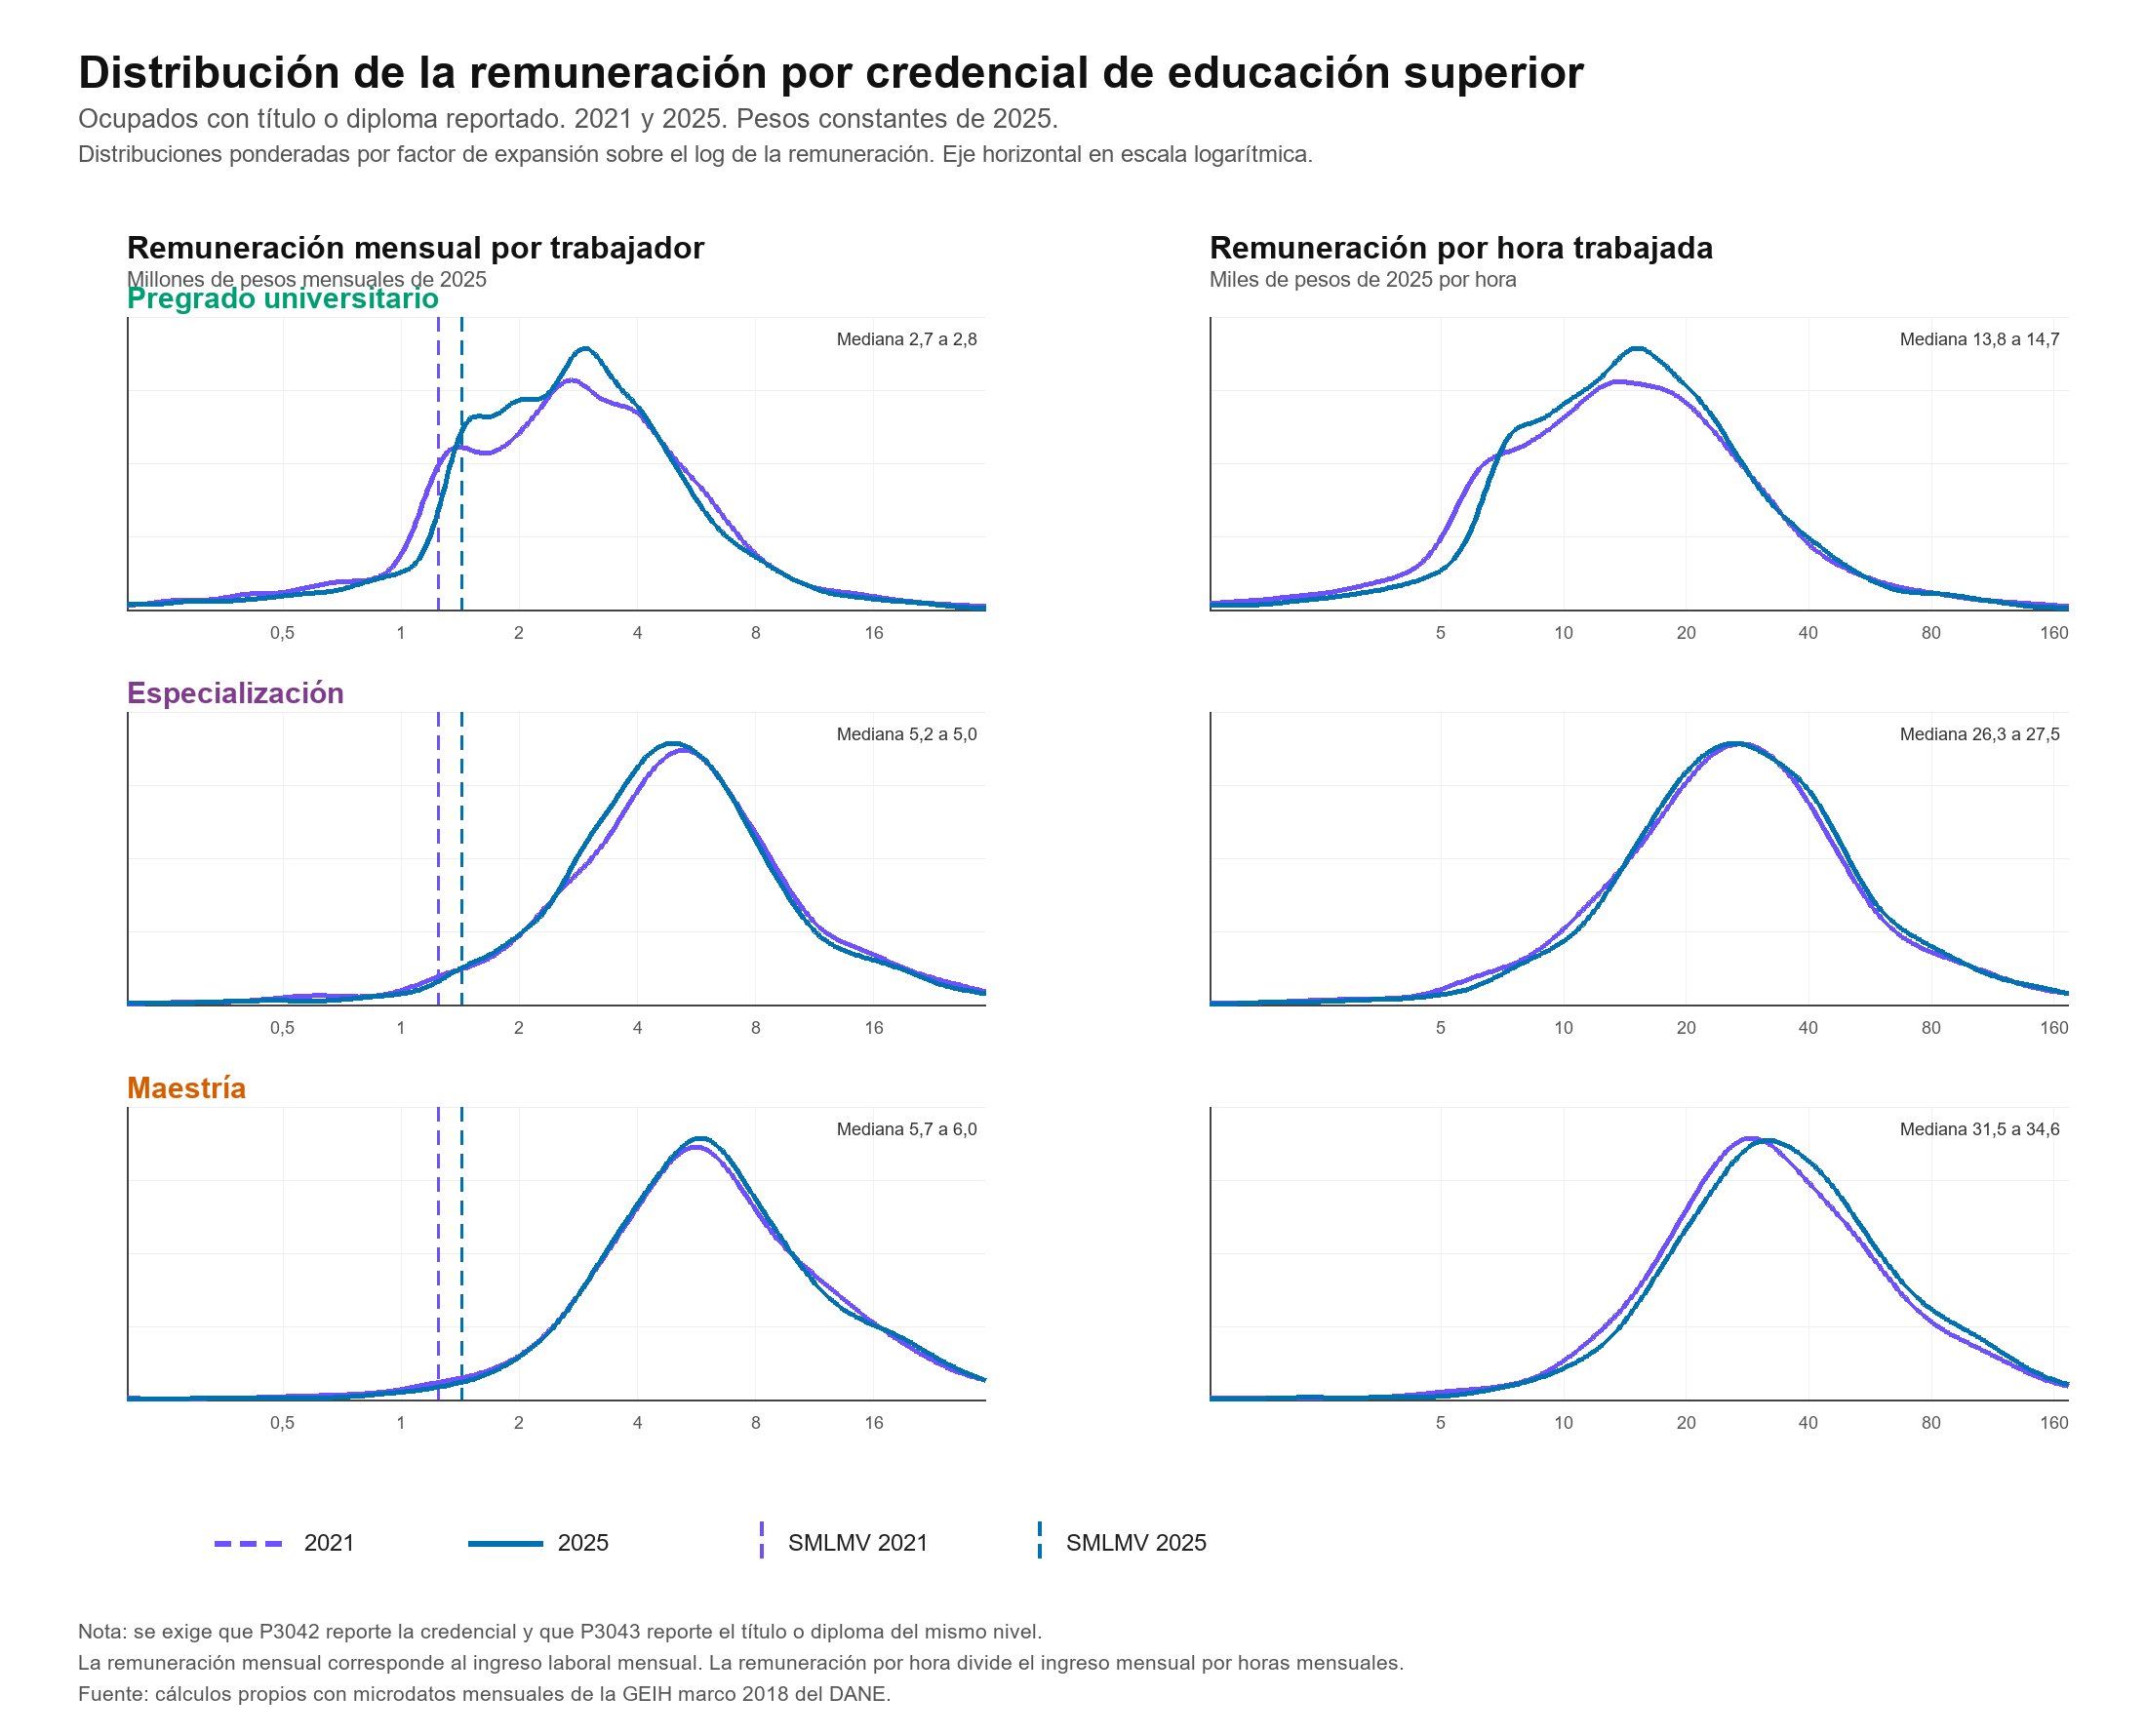
\includegraphics[width=0.98\textwidth]{Paper/figures/fig_kernel_remuneracion_credenciales_superiores_2021_2025.png}
  \caption{Distribución de la remuneración laboral por credencial de educación superior, 2021 y 2025}
  \label{fig:kernel_remuneracion_credenciales_superiores}
  \caption*{\footnotesize Nota: distribuciones estimadas con factores de expansión sobre el log de la remuneración. Se exige que P3042 reporte la credencial y que P3043 reporte el título o diploma del mismo nivel. El eje horizontal está en escala logarítmica. La remuneración mensual está en millones de pesos mensuales de 2025 y la remuneración por hora en miles de pesos de 2025 por hora. Fuente: cálculos propios con GEIH del DANE.}
\end{figure}

\begin{table}[H]
\centering
\caption{Aportes por logro educativo a la descomposición de la remuneración laboral, 2010--2025}
\label{tab:descomposicion_remuneracion_educacion_detalle}
\scriptsize
\begin{tabular}{@{}p{6.4cm}rr@{}}
\toprule
\multicolumn{3}{@{}l}{\textbf{Panel A. Remuneración mensual por trabajador}} \\
Factor & \shortstack{Aporte al cambio\\(miles de pesos\\mensuales de 2025)} & \shortstack{\% del\\cambio total} \\
\midrule
Productividad: Ninguno & 13,7 & 3,5\% \\
Productividad: Básica primaria & 23,6 & 6,0\% \\
Productividad: Básica secundaria & 5,1 & 1,3\% \\
Productividad: Educación media & 28,4 & 7,2\% \\
Productividad: Técnico o tecnológico & -2,2 & -0,6\% \\
Productividad: Pregrado universitario & -29,3 & -7,4\% \\
Productividad: Posgrado & -1,1 & -0,3\% \\
\textbf{Total productividad} & \textbf{38,1} & \textbf{9,6\%} \\
\addlinespace[0.35em]
Logro educativo: Ninguno & -88,9 & -22,5\% \\
Logro educativo: Básica primaria & -91,6 & -23,2\% \\
Logro educativo: Básica secundaria & -16,4 & -4,1\% \\
Logro educativo: Educación media & 113,4 & 28,7\% \\
Logro educativo: Técnico o tecnológico & 107,0 & 27,0\% \\
Logro educativo: Pregrado universitario & 174,1 & 44,0\% \\
Logro educativo: Posgrado & 160,0 & 40,4\% \\
\textbf{Total logro educativo} & \textbf{357,6} & \textbf{90,4\%} \\
\addlinespace[0.35em]
\addlinespace[0.6em]
\multicolumn{3}{@{}l}{\textbf{Panel B. Remuneración por hora trabajada}} \\
Factor & \shortstack{Aporte al cambio\\(pesos de 2025\\por hora)} & \shortstack{\% del\\cambio total} \\
\midrule
Productividad: Ninguno & 136 & 5,2\% \\
Productividad: Básica primaria & 234 & 8,9\% \\
Productividad: Básica secundaria & 45 & 1,7\% \\
Productividad: Educación media & 319 & 12,2\% \\
Productividad: Técnico o tecnológico & 41 & 1,6\% \\
Productividad: Pregrado universitario & -117 & -4,5\% \\
Productividad: Posgrado & 9 & 0,3\% \\
\textbf{Total productividad} & \textbf{669} & \textbf{25,6\%} \\
\addlinespace[0.35em]
Logro educativo: Ninguno & -474 & -18,1\% \\
Logro educativo: Básica primaria & -499 & -19,1\% \\
Logro educativo: Básica secundaria & -83 & -3,2\% \\
Logro educativo: Educación media & 566 & 21,6\% \\
Logro educativo: Técnico o tecnológico & 561 & 21,4\% \\
Logro educativo: Pregrado universitario & 978 & 37,4\% \\
Logro educativo: Posgrado & 898 & 34,3\% \\
\textbf{Total logro educativo} & \textbf{1.946} & \textbf{74,4\%} \\
\addlinespace[0.35em]
\bottomrule
\end{tabular}
\caption*{\footnotesize Nota: los aportes al cambio preservan el signo de cada contribución. Los porcentajes dividen cada factor por el cambio total del indicador correspondiente. Fuente: cálculos propios con GEIH del DANE.}
\end{table}


% Bloque desactivado: no se referencia en el cuerpo del documento.
\iffalse
\begin{table}[H]
\centering
\caption{Composición de los ocupados por logro educativo, sexo y formalidad, 2010 y 2025}
\label{tab:composicion_educacion_sexo_formalidad}
\footnotesize
\begin{tabular}{@{}p{4.2cm}rrrr@{}}
\toprule
\multicolumn{5}{@{}l}{\textbf{Panel A. Sexo}} \\
Logro educativo & Hombre 2010 & Mujer 2010 & Hombre 2025 & Mujer 2025 \\
\midrule
Primaria o menos & 67,8\% & 32,2\% & 70,0\% & 30,0\% \\
Secundaria o media & 59,7\% & 40,3\% & 61,7\% & 38,3\% \\
Superior o universitaria & 48,5\% & 51,5\% & 47,9\% & 52,1\% \\
\textbf{Total} & 60,1\% & 39,9\% & 58,8\% & 41,2\% \\
\addlinespace[0.6em]
\multicolumn{5}{@{}l}{\textbf{Panel B. Formalidad}} \\
Logro educativo & Formal 2010 & Informal 2010 & Formal 2025 & Informal 2025 \\
\midrule
Primaria o menos & 11,5\% & 88,5\% & 13,0\% & 87,0\% \\
Secundaria o media & 31,3\% & 68,7\% & 36,7\% & 63,3\% \\
Superior o universitaria & 67,5\% & 32,5\% & 76,0\% & 24,0\% \\
\textbf{Total} & 32,4\% & 67,6\% & 44,9\% & 55,1\% \\
\bottomrule
\end{tabular}
\caption*{\footnotesize Nota: participaciones dentro de cada logro educativo, calculadas con factores de expansión sobre la misma submuestra usada para medir remuneración. El Panel B clasifica como formal a quienes cotizan a pensión e informal a quienes no cotizan. Excluye observaciones sin clasificación formal/informal válida. Fuente: cálculos propios con GEIH del DANE.}
\end{table}
\fi

% Bloque desactivado: no se referencia en el cuerpo del documento.
\iffalse
\begin{table}[H]
\centering
\caption{Remuneración laboral por logro educativo y formalidad, 2010 y 2025}
\label{tab:remuneracion_educacion_formalidad}
\footnotesize
\begin{tabular}{@{}p{4.0cm}rrrr@{}}
\toprule
\multicolumn{5}{@{}l}{\textbf{Panel A. Remuneración mensual por trabajador (millones de pesos mensuales de 2025)}} \\
Logro educativo & Formal 2010 & Informal 2010 & Formal 2025 & Informal 2025 \\
\midrule
Primaria o menos & 1,43 & 0,80 & 1,71 & 0,89 \\
Secundaria & 1,62 & 0,99 & 1,79 & 1,08 \\
Universitaria o superior & 3,65 & 1,85 & 3,73 & 1,49 \\
\textbf{Total} & 2,55 & 1,00 & 2,89 & 1,08 \\
\addlinespace[0.7em]
\multicolumn{5}{@{}l}{\textbf{Panel B. Remuneración por hora trabajada (miles de pesos de 2025 por hora)}} \\
Logro educativo & Formal 2010 & Informal 2010 & Formal 2025 & Informal 2025 \\
\midrule
Primaria o menos & 6,1 & 4,1 & 8,1 & 4,9 \\
Secundaria & 7,1 & 4,9 & 8,7 & 5,8 \\
Universitaria o superior & 18,0 & 10,4 & 19,2 & 8,7 \\
\textbf{Total} & 11,8 & 5,1 & 14,5 & 5,9 \\
\bottomrule
\end{tabular}
\caption*{\footnotesize Nota: la clasificación formal corresponde a trabajadores ocupados que cotizan a pensión. La clasificación informal corresponde a quienes no cotizan. El cuadro excluye observaciones sin clasificación formal o informal válida. Fuente: cálculos propios con GEIH del DANE.}
\end{table}

\fi

% Bloque desactivado: no se referencia en el cuerpo del documento.
\iffalse
\begin{table}[H]
\centering
\caption{Remuneración laboral por logro educativo y grupo de edad, 2010 y 2025}
\label{tab:remuneracion_educacion_cohorte}
\scriptsize
\begin{tabular}{@{}p{3.6cm}p{1.6cm}rrr@{}}
\toprule
\multicolumn{5}{@{}l}{\textbf{Panel A. Remuneración mensual por trabajador (millones de pesos mensuales de 2025)}} \\
Logro educativo & Edad & 2010 & 2025 & Crec. anual \\
\midrule
Primaria o menos & 15--24 & 0,7 & 0,9 & 1,8\% \\
Primaria o menos & 25--34 & 0,9 & 1,0 & 0,9\% \\
Primaria o menos & 35--44 & 0,9 & 1,1 & 0,9\% \\
Primaria o menos & 45--54 & 0,9 & 1,1 & 1,2\% \\
Primaria o menos & 55 o más & 0,8 & 0,9 & 0,5\% \\
\addlinespace[0.3em]
Secundaria & 15--24 & 0,9 & 1,1 & 1,8\% \\
Secundaria & 25--34 & 1,2 & 1,4 & 1,0\% \\
Secundaria & 35--44 & 1,3 & 1,4 & 0,5\% \\
Secundaria & 45--54 & 1,4 & 1,4 & 0,2\% \\
Secundaria & 55 o más & 1,5 & 1,3 & -0,9\% \\
\addlinespace[0.3em]
Universitaria o superior & 15--24 & 1,3 & 1,6 & 1,2\% \\
Universitaria o superior & 25--34 & 2,6 & 2,7 & 0,2\% \\
Universitaria o superior & 35--44 & 3,5 & 3,7 & 0,3\% \\
Universitaria o superior & 45--54 & 4,4 & 4,0 & -0,6\% \\
Universitaria o superior & 55 o más & 4,8 & 4,1 & -1,1\% \\
\addlinespace[0.7em]
\multicolumn{5}{@{}l}{\textbf{Panel B. Remuneración por hora trabajada (miles de pesos de 2025 por hora)}} \\
Logro educativo & Edad & 2010 & 2025 & Crec. anual \\
\midrule
Primaria o menos & 15--24 & 3,4 & 4,8 & 2,3\% \\
Primaria o menos & 25--34 & 4,3 & 5,4 & 1,5\% \\
Primaria o menos & 35--44 & 4,5 & 5,6 & 1,5\% \\
Primaria o menos & 45--54 & 4,4 & 5,8 & 1,8\% \\
Primaria o menos & 55 o más & 4,4 & 5,1 & 1,0\% \\
\addlinespace[0.3em]
Secundaria & 15--24 & 4,4 & 6,1 & 2,2\% \\
Secundaria & 25--34 & 5,4 & 6,9 & 1,7\% \\
Secundaria & 35--44 & 6,1 & 7,2 & 1,1\% \\
Secundaria & 45--54 & 6,5 & 7,2 & 0,7\% \\
Secundaria & 55 o más & 7,8 & 7,3 & -0,5\% \\
\addlinespace[0.3em]
Universitaria o superior & 15--24 & 7,4 & 9,1 & 1,4\% \\
Universitaria o superior & 25--34 & 13,1 & 14,1 & 0,5\% \\
Universitaria o superior & 35--44 & 17,8 & 19,0 & 0,5\% \\
Universitaria o superior & 45--54 & 23,0 & 21,3 & -0,5\% \\
Universitaria o superior & 55 o más & 27,2 & 23,4 & -1,0\% \\
\bottomrule
\end{tabular}
\caption*{\footnotesize Nota: el crecimiento es anualizado para 2010--2025. Los grupos de edad comparan personas del mismo rango etario observadas en cada año. No siguen una misma cohorte de nacimiento a lo largo del tiempo. Fuente: cálculos propios con GEIH del DANE.}
\end{table}


\begin{table}[H]
\centering
\caption{Remuneración laboral por cohorte de nacimiento y logro educativo, 2010 y 2025}
\label{tab:remuneracion_educacion_cohortes_nacimiento}
\scriptsize
\begin{tabular}{@{}p{2.0cm}p{3.5cm}rrr@{}}
\toprule
\multicolumn{5}{@{}l}{\textbf{Panel A. Remuneración mensual por trabajador (millones de pesos mensuales de 2025)}} \\
Cohorte & Logro educativo & 2010 & 2025 & Crec. anual \\
\midrule
1985--1990 & \textbf{Total} & 1,16 & 2,26 & 4,54\% \\
1985--1990 & Primaria o menos & 0,75 & 1,08 & 2,49\% \\
1985--1990 & Secundaria & 1,03 & 1,40 & 2,05\% \\
1985--1990 & Universitaria o superior & 1,63 & 3,69 & 5,61\% \\
\addlinespace[0.4em]
1980--1985 & \textbf{Total} & 1,52 & 2,22 & 2,58\% \\
1980--1985 & Primaria o menos & 0,85 & 1,06 & 1,54\% \\
1980--1985 & Secundaria & 1,15 & 1,44 & 1,51\% \\
1980--1985 & Universitaria o superior & 2,48 & 3,82 & 2,92\% \\
\addlinespace[0.4em]
1975--1980 & \textbf{Total} & 1,67 & 2,17 & 1,77\% \\
1975--1980 & Primaria o menos & 0,97 & 1,11 & 0,90\% \\
1975--1980 & Secundaria & 1,21 & 1,42 & 1,07\% \\
1975--1980 & Universitaria o superior & 3,02 & 4,11 & 2,07\% \\
\addlinespace[0.8em]
\multicolumn{5}{@{}l}{\textbf{Panel B. Remuneración por hora trabajada (miles de pesos de 2025 por hora)}} \\
Cohorte & Logro educativo & 2010 & 2025 & Crec. anual \\
\midrule
1985--1990 & \textbf{Total} & 5,7 & 11,6 & 4,87\% \\
1985--1990 & Primaria o menos & 3,6 & 5,7 & 3,02\% \\
1985--1990 & Secundaria & 4,9 & 7,0 & 2,52\% \\
1985--1990 & Universitaria o superior & 8,6 & 19,2 & 5,49\% \\
\addlinespace[0.4em]
1980--1985 & \textbf{Total} & 7,2 & 11,5 & 3,12\% \\
1980--1985 & Primaria o menos & 4,1 & 5,6 & 2,22\% \\
1980--1985 & Secundaria & 5,3 & 7,3 & 2,15\% \\
1980--1985 & Universitaria o superior & 12,4 & 19,9 & 3,19\% \\
\addlinespace[0.4em]
1975--1980 & \textbf{Total} & 8,0 & 11,3 & 2,34\% \\
1975--1980 & Primaria o menos & 4,7 & 5,8 & 1,49\% \\
1975--1980 & Secundaria & 5,6 & 7,3 & 1,73\% \\
1975--1980 & Universitaria o superior & 15,1 & 21,6 & 2,44\% \\
\bottomrule
\end{tabular}
\caption*{\footnotesize Nota: los rangos de cohorte son intervalos de cinco años. Por ejemplo, 1985--1990 incluye nacidos de 1985 a 1989. Se reportan las cohortes que aparecen tanto en 2010 como en 2025 dentro de los rangos solicitados. El crecimiento es anualizado para 2010--2025. Fuente: cálculos propios con GEIH del DANE.}
\end{table}

\fi

% Bloque desactivado: no se referencia en el cuerpo del documento.
\iffalse
\begin{table}[H]
\centering
\caption{Remuneración laboral de ocupados de 25 a 29 años con educación universitaria o superior, 2010 y 2025}
\label{tab:remuneracion_recien_graduados}
\footnotesize
\begin{tabular}{@{}p{6.6cm}rrr@{}}
\toprule
Indicador & 2010 & 2025 & Crec. anual \\
\midrule
Ocupados (millones de personas) & 0,73 & 1,27 & 3,73\% \\
Remuneración mensual por trabajador (millones de pesos de 2025) & 2,33 & 2,40 & 0,18\% \\
Remuneración por hora trabajada (miles de pesos de 2025) & 11,7 & 12,7 & 0,51\% \\
\bottomrule
\end{tabular}
\caption*{\footnotesize Nota: la GEIH no identifica si la persona acaba de graduarse ni el año de graduación. Este cuadro aproxima la remuneración de recién graduados con personas ocupadas de 25 a 29 años que reportan educación universitaria o superior. Por lo tanto, debe leerse como una aproximación a jóvenes con educación superior, no como graduados observados directamente. El crecimiento es anualizado para 2010--2025. La serie excluye 2020. Fuente: cálculos propios con GEIH del DANE.}
\end{table}

\fi

% Bloque desactivado: no se referencia en el cuerpo del documento.
\iffalse
\begin{figure}[H]
  \centering
  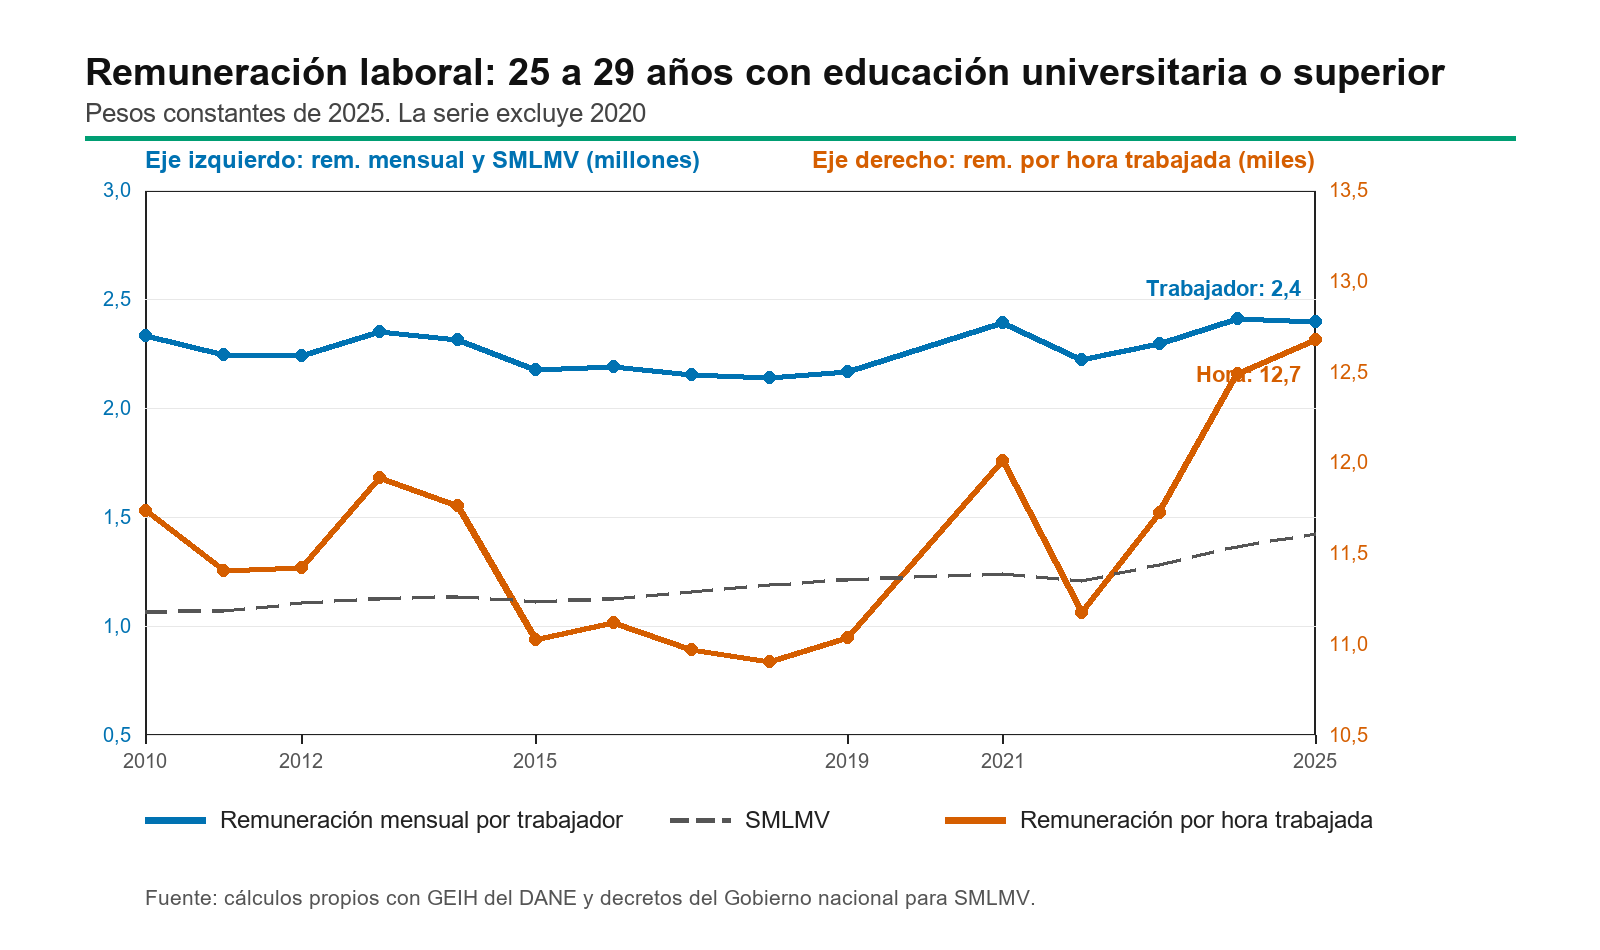
\includegraphics[width=0.96\textwidth]{Paper/figures/fig_remuneracion_recien_graduados_series.png}
  \caption{Evolución de la remuneración laboral de ocupados de 25 a 29 años con educación superior, 2010--2025}
  \label{fig:remuneracion_recien_graduados_series}
  \caption*{\footnotesize Nota: el eje izquierdo muestra la remuneración mensual por trabajador y el SMLMV, ambos en millones de pesos mensuales de 2025. El eje derecho muestra la remuneración por hora trabajada en miles de pesos de 2025. La GEIH no identifica si la persona acaba de graduarse ni el año de graduación. El grupo de 25 a 29 años con educación superior se usa como aproximación a recién graduados. El SMLMV no incluye auxilio de transporte. La serie excluye 2020. Fuente: cálculos propios con GEIH del DANE y decretos del Gobierno nacional para SMLMV.}
\end{figure}
\fi

% Bloque desactivado: no se referencia en el cuerpo del documento.
\iffalse
\begin{figure}[H]
  \centering
  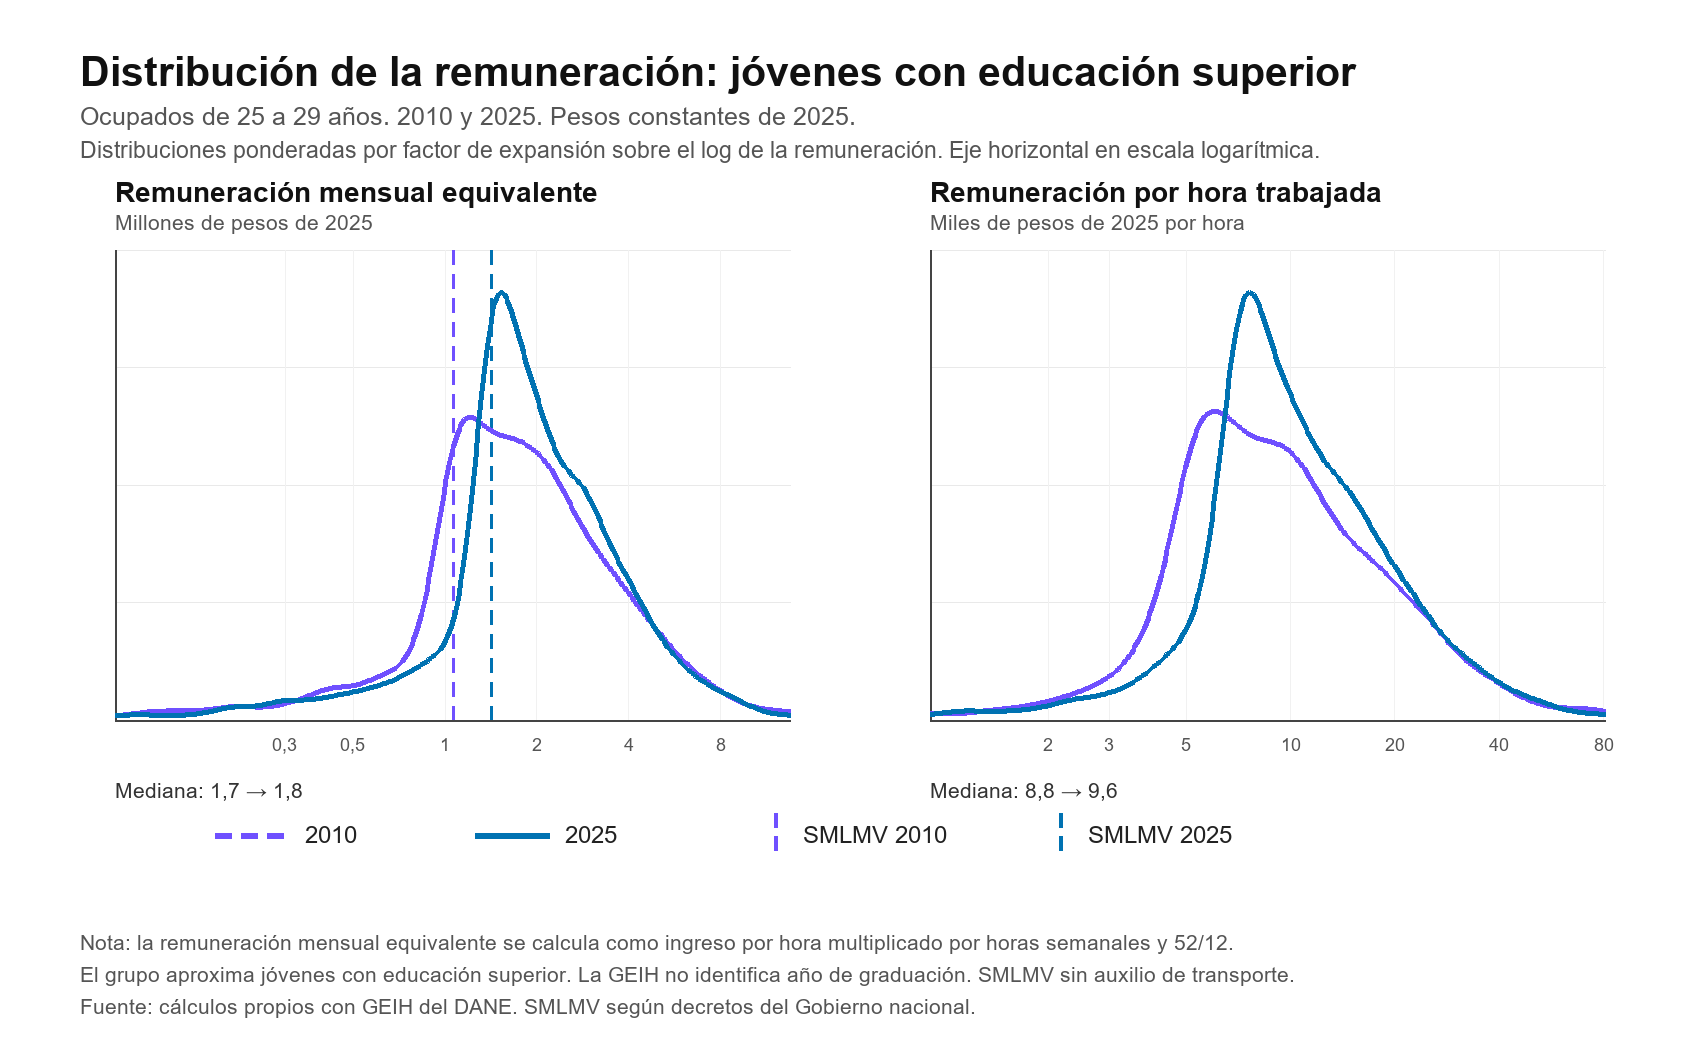
\includegraphics[width=0.98\textwidth]{Paper/figures/fig_kernel_remuneracion_universitaria_25_29_2010_2025.png}
  \caption{Distribución de la remuneración laboral de ocupados de 25 a 29 años con educación superior, 2010 y 2025}
  \label{fig:kernel_remuneracion_universitaria_25_29}
  \caption*{\footnotesize Nota: distribuciones estimadas con factores de expansión sobre el log de la remuneración. El eje horizontal está en escala logarítmica. La GEIH no identifica si la persona acaba de graduarse ni el año de graduación. El grupo de 25 a 29 años con educación superior se usa como aproximación a recién graduados. El SMLMV no incluye auxilio de transporte. Fuente: cálculos propios con GEIH del DANE y decretos del Gobierno nacional para SMLMV.}
\end{figure}
\fi
